\documentclass[12pt]{article}
\usepackage{etex}

\usepackage{pstricks,amssymb,amsfonts,amsmath,array,multicol,moreverb,color}
\usepackage{DraTex,AlDraTex}
\usepackage{graphicx}
\usepackage{fancyhdr}

\input{mydef1.tex}
\input{circuits.tex}
\input{signals.tex}

\mathchardef\scriptT="0254  %Script T for transform
\def\endex{\hfill$\sqcap\hskip-8pt\sqcup$}

\topmargin=-0.5in
\textheight=8.875in
\oddsidemargin=0in
\textwidth=6.5in
%\pagestyle{empty}     %Comment out to obtain page numbering
%\headheight=14.5pt
%\pagestyle{fancy}
\renewcommand{\thesubsection}{\arabic{subsection}}

\definecolor{black}{gray}{0}
\definecolor{gray}{gray}{0.7}
\definecolor{red}{rgb}{1,0,0}
\definecolor{green}{rgb}{0,1,0}
\definecolor{blue}{rgb}{0,0,1}
\definecolor{white}{rgb}{1,1,1}
\definecolor{yellow}{rgb}{1,1,0.5}
\definecolor{magenta}{rgb}{1,0,1}
\definecolor{cyan}{rgb}{0,1,1}

\begin{document}
%started 10-18-13, PM
%updated 11-09-15, PM
%updated 09-21-16, PM

%\begin{large}
%\noindent ECEN 4242\hfill Communication Theory\hfill Fall 2016\par
%\end{large}
%\smallskip

%\noindent 9-21-16\hfill P.~Mathys\par
%\smallskip

%\hrule
%\bigskip

%\subsection*{Appendix A: Laplace Transform Tables}
\begin{large}
\textbf{Laplace Transform Tables}
\end{large}
\bigskip

\begin{footnotesize}
\begin{center}
\begin{tabular}{!{\vrule width 1pt}l|ccc!{\vrule width 1pt}}
\noalign{\hrule height1pt}
\multicolumn{4}{!{\vrule width 1pt}c!{\vrule width 1pt}}{\phantom{m}}\\[-11pt]
\multicolumn{4}{!{\vrule width 1pt}c!{\vrule width 1pt}}
{\strut\textbf{Specific Unilateral Laplace Transform Pairs}}\\[2pt]
\hline
\phantom{m}&&&\\[-10pt]
Signal&$x(t)=\scriptL^{-1}[X(s)]$&&$X(s)=\int_0^{\infty} x(t) e^{-st}dt$\\[3pt]
\noalign{\hrule height1pt}
\phantom{m}&&&\\[-10pt]
Unit impulse&$\delta(t)$&$\Longleftrightarrow$
&$1$\\[5pt]
Unit step&$u(t)=\left\{\begin{array}{ll}1,&t>0\\0,&t<0\end{array}\right.$&$\Longleftrightarrow$
&$\displaystyle\frac{1}{s}$\\[11pt]
Exponential&$e^{-\alpha t}\,u(t)$&$\Longleftrightarrow$
&$\displaystyle\frac{1}{s+\alpha}$\\[10pt]
Power of $t$&$t^n\,u(t)$&$\Longleftrightarrow$
&$\displaystyle\frac{n!}{s^{n+1}}$\\[10pt]
Damped power of $t$&$t^n\,e^{-\alpha t}\,u(t)$&$\Longleftrightarrow$
&$\displaystyle\frac{n!}{(s+\alpha)^{n+1}}$\\[10pt]
Sine&$\sin(\beta t)\,u(t)$&$\Longleftrightarrow$
&$\displaystyle\frac{\beta}{s^2+\beta^2}$\\[10pt]
Cosine&$\cos(\beta t)\,u(t)$&$\Longleftrightarrow$
&$\displaystyle\frac{s}{s^2+\beta^2}$\\[10pt]
Damped sine&$e^{-\alpha t}\,\sin(\beta t)\,u(t)$&$\Longleftrightarrow$
&$\displaystyle\frac{\beta}{(s+\alpha)^2+\beta^2}$\\[10pt]
Damped cosine&$e^{-\alpha t}\,\cos(\beta t)\,u(t)$&$\Longleftrightarrow$
&$\displaystyle\frac{s+\alpha}{(s+\alpha)^2+\beta^2}$\\[12pt]
$\begin{subarray}{l}\displaystyle\mbox{$t$ times}\\[4pt]\displaystyle\mbox{damped sine}\end{subarray}$&
$t\,e^{-\alpha t}\,\sin(\beta t)\,u(t)$&$\Longleftrightarrow$
&$\displaystyle\frac{2\beta\,(s+\alpha)}{((s+\alpha)^2+\beta^2)^2}$\\[12pt]
$\begin{subarray}{l}\displaystyle\mbox{$t$ times}\\[4pt]\displaystyle\mbox{damped cosine}\end{subarray}$&
$t\,e^{-\alpha t}\,\cos(\beta t)\,u(t)$&$\Longleftrightarrow$
&$\displaystyle\frac{(s+\alpha)^2-\beta^2}{((s+\alpha)^2+\beta^2)^2}$\\[12pt]
\noalign{\hrule height1pt}
\end{tabular}
\end{center}
\medskip

\begin{center}
\begin{tabular}{!{\vrule width 1pt}l|ccc!{\vrule width 1pt}}
\noalign{\hrule height1pt}
\multicolumn{4}{!{\vrule width 1pt}c!{\vrule width 1pt}}{\phantom{m}}\\[-11pt]
\multicolumn{4}{!{\vrule width 1pt}c!{\vrule width 1pt}}
{\strut\textbf{Unilateral Laplace Transform Properties}}\\[2pt]
\hline
\phantom{m}&&&\\[-10pt]
Property&$x(t)=\scriptL^{-1}[X(s)]$&&$X(s)=\int_0^{\infty} x(t) e^{-st}dt$\\[3pt]
\noalign{\hrule height1pt}
\phantom{m}&&&\\[-10pt]
Linearity&$A x_1(t)+B x_2(t)$&$\Longleftrightarrow$
&$A X_1(s)+B X_2(s)$\\[5pt]
Scale change&$x(at)$&$\Longleftrightarrow$
&$\displaystyle\frac{1}{a}\,X\left(\frac{s}{a}\right),\ a>0$\\[10pt]
Time shift&$x(t-T)\,u(t-T)$&$\Longleftrightarrow$
&$e^{-sT}\,X(s),\ T>0$\\[5pt]
$s$-shift&$e^{-\alpha t}\,x(t)$&$\Longleftrightarrow$
&$X(s+\alpha)$\\[5pt]
Differentiation&$\displaystyle\frac{dx(t)}{dt}$&$\Longleftrightarrow$
&$s\,X(s)-x(0^{-})$\\[8pt]
%&$\displaystyle\frac{d^n x(t)}{dt^n}=x^{(n)}(t)$&$\Longleftrightarrow$
%&$s^n\,X(s)-\sum_{i=0}^{n-1} s^{n-i-1}\,x^{(i)}(0^{-})$\\[10pt]
Times $t$&$t\,x(t)$&$\Longleftrightarrow$
&$\displaystyle\frac{-dX(s)}{ds}$\\[10pt]
Integration&$\int_0^t x(\tau)\,d\tau$&$\Longleftrightarrow$
&$\displaystyle\frac{X(s)}{s}$\\[10pt]
Convolution&$\int_0^t x_1(\tau)\,x_2(t-\tau)\,d\tau$&$\Longleftrightarrow$
&$X_1(s)\,X_2(s)$\\[6pt]
Conjugation&$x^*(t)$&$\Longleftrightarrow$
&$X^*(s^*)$\\[5pt]
$\begin{subarray}{l}\displaystyle\text{Initial value}\\[3pt]\displaystyle\text{(if it exists)}\end{subarray}$&
$x(0^{+})$&$\Longleftrightarrow$
&$\lim\limits_{s\rightarrow\infty}\> s\,X(s)$\\[9pt]
$\begin{subarray}{l}\displaystyle\text{Final value}\\[3pt]\displaystyle\text{(if it exists)}\end{subarray}$&
$x(\infty)$&$\Longleftrightarrow$
&$\lim\limits_{s\rightarrow 0}\> s\,X(s)$\\[9pt]
\noalign{\hrule height1pt}
\end{tabular}
\end{center}
\end{footnotesize}
\vfill
\eject

%\subsection*{Appendix C: Fourier Transform Tables}
\begin{large}
\textbf{Fourier Transform Tables}
\end{large}
\bigskip

\begin{footnotesize}
\begin{center}
\begin{tabular}{!{\vrule width 1pt}l|ccc!{\vrule width 1pt}}
\noalign{\hrule height1pt}
\multicolumn{4}{!{\vrule width 1pt}c!{\vrule width 1pt}}{\phantom{m}}\\[-11pt]
\multicolumn{4}{!{\vrule width 1pt}c!{\vrule width 1pt}}
{\strut\textbf{Specific Fourier Transform Pairs}}\\[2pt]
\hline
\phantom{m}&&&\\[-10pt]
Signal&$x(t)=\int_{-\infty}^{\infty} X(f)e^{j2\pi ft}df$&&$X(f)=\int_{-\infty}^{\infty} x(t) e^{-j2\pi ft} dt$\\[6pt]
\noalign{\hrule height1pt}
\phantom{m}&&&\\[-10pt]
Unit Impulse&$\delta(t)$&$\Longleftrightarrow$&$1$\\[5pt]
Constant&$1$&$\Longleftrightarrow$&$\delta(f)$\\[5pt]
Unit Step&$u(t)=\displaystyle\left\{\begin{array}{ll}1,&t> 0\\
0,&t< 0\end{array}\right.$&$\Longleftrightarrow$
&$\displaystyle\frac{\delta(f)}{2}+\frac{1}{j2\pi f}$\\[14pt]
Signum&$\sgn(t)=\displaystyle\left\{\begin{array}{ll}\phantom{-}1,&t>0\\\phantom{-}0,&t=0\\
-1,&t< 0\end{array}\right.$&$\Longleftrightarrow$
&$\displaystyle\frac{1}{j\pi f}$\\[20pt]
$\begin{subarray}{l}\displaystyle\text{Exponential}\\[4pt]\displaystyle\text{1-sided}\end{subarray}$&
$e^{-at} u(t)$&$\Longleftrightarrow$
&$\displaystyle\frac{1}{a+j2\pi f}$\\[14pt]
Gaussian&$e^{-\pi t^2}$&$\Longleftrightarrow$&$e^{-\pi f^2}$\\[8pt]
Sine&$\sin(2\pi f_0 t)$&$\Longleftrightarrow$&$
\displaystyle\frac{\delta(f{-}f_0)-\delta(f{+}f_0)}{2j}$\\[14pt]
Cosine&$\cos(2\pi f_0 t)$&$\Longleftrightarrow$&$
\displaystyle\frac{\delta(f{-}f_0)+\delta(f{+}f_0)}{2}$\\[14pt]
Sine ($t>0$)&$\sin(2\pi f_0 t)\,u(t)$&$\Longleftrightarrow$&$
\displaystyle\frac{\delta(f{-}f_0)-\delta(f{+}f_0)}{4j}+\frac{1}{2\pi}\,\frac{f_0}{f_0^2-f^2}$\\[14pt]
Cosine ($t>0$)&$\cos(2\pi f_0 t)\,u(t)$&$\Longleftrightarrow$&$
\displaystyle\frac{\delta(f{-}f_0)+\delta(f{+}f_0)}{4}+\frac{1}{j2\pi}\,\frac{f}{f^2-f_0^2}$\\[14pt]
Rectangular&$x(t)=\displaystyle\left\{\begin{array}{ll}1,&|t|< \tau/2\\
0,&\mbox{otherwise}\end{array}\right.$&$\Longleftrightarrow$
&$\displaystyle\frac{\sin(\pi f\tau)}{\pi f}$\\[14pt]
``sin x over x''&$\displaystyle \frac{\sin(2\pi Wt)}{\pi t}$
&$\Longleftrightarrow$&$X(f)=\displaystyle\left\{\begin{array}{ll}1,&|f|<W\\
0,&\mbox{otherwise}\end{array}\right.$\\[12pt]
$\begin{subarray}{l}\displaystyle\text{Hilbert}\\[4pt]\displaystyle\text{Transform}\end{subarray}$&
$\displaystyle\frac{1}{\pi t}$&$\Longleftrightarrow$
&$-j\sgn(f)$\\[12pt]
Tone FM&$\displaystyle e^{j\beta\sin(2\pi f_m t)}
=\sum_{k=-\infty}^{\infty} J_k(\beta)\,e^{j2\pi k f_m t}$&$\Longleftrightarrow$
&$\displaystyle\sum_{k=-\infty}^{\infty} J_k(\beta)\>\delta(f-k f_m)$\\[16pt]
Pulse Train&$\displaystyle\sum_{m=-\infty}^{\infty} \delta(t-mT)$&$\Longleftrightarrow$
&$\displaystyle\frac{1}{T}\sum_{k=-\infty}^{\infty} \delta\big(f-\frac{k}{T}\big)$\\[16pt]
\noalign{\hrule height1pt}
\end{tabular}
\end{center}
\bigskip

\noindent Bessel function, 1'st kind, order $k$:
$\displaystyle J_k(\beta)=\frac{1}{2\pi}\int_{-\pi}^{\pi}e^{j(\beta\sin x-kx)}\,dx.$
\medskip

\begin{center}
\begin{tabular}{!{\vrule width 1pt}l|ccc!{\vrule width 1pt}}
\noalign{\hrule height1pt}
\multicolumn{4}{!{\vrule width 1pt}c!{\vrule width 1pt}}{\phantom{m}}\\[-11pt]
\multicolumn{4}{!{\vrule width 1pt}c!{\vrule width 1pt}}
{\strut\textbf{Fourier Transform Properties}}\\[2pt]
\hline
\phantom{m}&&&\\[-10pt]
Property&$x(t)=\int_{-\infty}^{\infty} X(f)e^{j2\pi ft}df$&&$X(f)=\int_{-\infty}^{\infty} x(t) e^{-j2\pi ft} dt$\\[6pt]
\noalign{\hrule height1pt}
\phantom{m}&&&\\[-9pt]
Linearity&$A x_1(t)+B x_2(t)$&$\Longleftrightarrow$
&$A X_1(f)+B X_2(f)$\\[5pt]
Duality&$X(t)$&$\Longleftrightarrow$
&$x(-f)$\\[5pt]
Scale Change&$x(at),\>\ a\ne 0$&$\Longleftrightarrow$
&$\displaystyle \frac{1}{|a|}\,X\Big(\frac{f}{a}\Big)$\\[12pt]
Time Shift&$x(t-t_0)$&$\Longleftrightarrow$
&$X(f)\,e^{-j2\pi f t_0}$\\[6pt]
Frequency Shift&$x(t)\,e^{j2\pi f_0 t}$
&$\Longleftrightarrow$&$X(f-f_0)$\\[6pt]
Convolution&$\int_{-\infty}^{\infty} x(\tau)\,h(t-\tau)\,d\tau$&$\Longleftrightarrow$
&$X(f)\,H(f)$\\[6pt]
Multiplication&$v(t)\,w(t)$&$\Longleftrightarrow$
&$\int_{-\infty}^{\infty} V(\mu)\,W(f-\mu)\,d\mu$\\[6pt]
Differentiation&$\displaystyle \frac{dx(t)}{dt}$&$\Longleftrightarrow$
&$j2\pi f\, X(f)$\\[6pt]
Times $t$&$t\,x(t)$&$\Longleftrightarrow$
&$\displaystyle\frac{-1}{j2\pi}\,\frac{dX(f)}{df}$\\[12pt]
Integration&$\displaystyle\int_{-\infty}^t x(\tau)\,d\tau$&$\Longleftrightarrow$
&$\displaystyle\frac{X(f)}{j2\pi f}+\frac{X(0)}{2}\,\delta(f)$\\[16pt]
Even Symmetry&$x(t)=x(-t)$&$\Longleftrightarrow$
&$X(f)=X(-f)$\\[6pt]
Odd Symmetry&$x(t)=-x(-t)$&$\Longleftrightarrow$
&$X(f)=-X(-f)$\\[7pt]
Real $x(t)$&$x(t)=x^*(t)$&$\Longleftrightarrow$
&$\begin{subarray}{c}\displaystyle X(f)=X^*(-f)\\[3pt]
\displaystyle\text{($|X(f)|$ even, $\angle X(f)$ odd)}\end{subarray}$\\[12pt]
$\begin{subarray}{l}\displaystyle\text{Periodic $x(t)$}\\[4pt]\displaystyle\text{($X_k$: FS Coefficients)}\end{subarray}$
&$\displaystyle\sum_{k=-\infty}^{\infty} X_k\,e^{j2\pi kt/T_1}$&$\Longleftrightarrow$
&$\displaystyle\sum_{k=-\infty}^{\infty} X_k\,\delta\big(f{-}\frac{k}{T_1}\big)$\\[16pt]
Parseval&$\int_{-\infty}^{\infty} |x(t)|^2\,dt$&$=$
&$\int_{-\infty}^{\infty} |X(f)|^2\,df$\\[8pt]
\noalign{\hrule height1pt}
\end{tabular}
\end{center}
\bigskip

\noindent Fourier series (period $T_1$): $\displaystyle X_k=\frac{1}{T_1}\int_{T_1}
x(t)\,e^{-j2\pi kt/T_1}\,dt \quad\Longleftrightarrow\quad
x(t)=\sum_{k=-\infty}^{\infty} X_k e^{j2\pi kt/T_1}$.
\end{footnotesize}
\vfill
\eject

%\subsection*{Appendix D: Fourier Series Tables}
\begin{large}
\textbf{Fourier Series Tables}
\end{large}
\bigskip

\begin{footnotesize}
\begin{center}
\begin{tabular}{!{\vrule width 1pt}l|ccc!{\vrule width 1pt}}
\noalign{\hrule height1pt}
\multicolumn{4}{!{\vrule width 1pt}c!{\vrule width 1pt}}{\phantom{m}}\\[-9pt]
\multicolumn{4}{!{\vrule width 1pt}c!{\vrule width 1pt}}
{\strut\textbf{Specific Fourier Series Pairs}, $T_1$: Period}\\[4pt]
\hline
\phantom{m}&&&\\[-10pt]
Signal&$\displaystyle x(t)=\sum_{k=-\infty}^{\infty} X_k\,e^{j2\pi kt/T_1}$&
&$\displaystyle X_k=\frac{1}{T_1}\int_{T_1} x(t)\,e^{-j2\pi kt/T_1}\,dt$\\[16pt]
\noalign{\hrule height1pt}
\phantom{m}&&&\\[-10pt]
Unit Impulse&$\delta(t)$&$\Longleftrightarrow$&$\displaystyle\frac{1}{T_1}$\\[12pt]
Constant&$1$&$\Longleftrightarrow$&$\displaystyle\frac{\sin(\pi k)}{\pi k}
=\displaystyle\left\{\begin{array}{ll}1,&k=0\\0,&\mbox{otherwise}\end{array}\right.$\\[16pt]
$\begin{subarray}{l}\displaystyle\text{Complex}\\[4pt]\displaystyle\text{Exponential}\end{subarray}$&
$e^{\pm j2\pi mt/T_1}$&$\Longleftrightarrow$
&$\displaystyle\frac{\sin(\pi (k\mp m))}{\pi (k\mp m)}
=\displaystyle\left\{\begin{array}{ll}1,&k=\pm m\\0,&\mbox{otherwise}\end{array}\right.$\\[16pt]
Sine, $\displaystyle f=\frac{m}{T_1}$&$\sin(2\pi mt/T_1)$&$\Longleftrightarrow$
&$\displaystyle\left\{\begin{array}{ll}1/(2j),&k=m\\-1/(2j),&k=-m\\0,&\mbox{otherwise}\end{array}\right.$\\[24pt]
Cosine, $\displaystyle f=\frac{m}{T_1}$&$\cos(2\pi mt/T_1)$&$\Longleftrightarrow$&$
\displaystyle\left\{\begin{array}{ll}1/2,&|k|=m\\0,&\mbox{otherwise}\end{array}\right.$\\[14pt]
Rectangular&$x(t)=\displaystyle\left\{\begin{array}{ll}1,&|t|< \tau/2\\
0,&\mbox{otherwise}\end{array}\right.$&$\Longleftrightarrow$
&$\displaystyle\frac{\sin(\pi k\tau/T_1)}{\pi k}$\\[12pt]
\noalign{\hrule height1pt}
\end{tabular}
\end{center}
\medskip

\begin{center}
\begin{tabular}{!{\vrule width 1pt}l|ccc!{\vrule width 1pt}}
\noalign{\hrule height1pt}
\multicolumn{4}{!{\vrule width 1pt}c!{\vrule width 1pt}}{\phantom{m}}\\[-9pt]
\multicolumn{4}{!{\vrule width 1pt}c!{\vrule width 1pt}}
{\strut\textbf{Fourier Series Properties}, $T_1$: Period}\\[4pt]
\hline
\phantom{m}&&&\\[-10pt]
Property&$\displaystyle x(t)=\sum_{k=-\infty}^{\infty} X_k\,e^{j2\pi kt/T_1}$&
&$\displaystyle X_k=\frac{1}{T_1}\int_{T_1} x(t)\,e^{-j2\pi kt/T_1}\,dt$\\[16pt]
\noalign{\hrule height1pt}
\phantom{m}&&&\\[-9pt]
Linearity&$A x_1(t)+B x_2(t)$&$\Longleftrightarrow$
&$A X_1[k]+B X_2[k]$\\[5pt]
Scale Change&$x(at),\ \ \big(x(t)=0,\ |t|\ge\frac{T_1}{a}\big)$&$\Longleftrightarrow$
&$\displaystyle \frac{1}{|a|}\,X[k/a],\ \ a\ne 0$\\[12pt]
Time Shift&$x(t-t_0)$&$\Longleftrightarrow$
&$X_k\,e^{-j2\pi kt_0/T_1}$\\[6pt]
Frequency Shift&$x(t)\,e^{j2\pi k_0 t/T_1}$
&$\Longleftrightarrow$&$X_{k-k_0}$\\[6pt]
Convolution&$\displaystyle\frac{1}{T_1}\int_{T_1} x(\tau)\,h(t-\tau)\,d\tau$&$\Longleftrightarrow$
&$X_k\,H_k$\\[10pt]
Multiplication&$v(t)\,w(t)$&$\Longleftrightarrow$
&$\displaystyle\sum_{m=-\infty}^{\infty} V_m\,W_{k-m}$\\[14pt]
Even Symmetry&$x(t)=x(-t)$&$\Longleftrightarrow$
&$X_k=X_{-k}$\\[6pt]
Odd Symmetry&$x(t)=-x(-t)$&$\Longleftrightarrow$
&$X_k=-X_{-k}$\\[6pt]
Real $x(t)$&$x(t)=x^*(t)$&$\Longleftrightarrow$
&$\begin{subarray}{c}\displaystyle X_k=X^*_{-k}\\[3pt]
\displaystyle\text{($|X_k|$ even, $\angle X_k$ odd)}\end{subarray}$\\[12pt]
Parseval&$\displaystyle\frac{1}{T_1}\int_{T_1} |x(t)|^2\,dt$&$=$
&$\displaystyle\sum_{k=-\infty}^{\infty} |X_k|^2$\\[14pt]
\noalign{\hrule height1pt}
\end{tabular}
\end{center}
\end{footnotesize}

\vfill
\eject

%\subsection*{Appendix E: Discrete-Time Fourier Transform Tables}
\begin{large}
\textbf{Discrete-Time Fourier Transform Tables}
\end{large}
\bigskip

\begin{footnotesize}
\begin{center}
\begin{tabular}{!{\vrule width 1pt}l|ccc!{\vrule width 1pt}}
\noalign{\hrule height1pt}
\multicolumn{4}{!{\vrule width 1pt}c!{\vrule width 1pt}}{\phantom{m}}\\[-11pt]
\multicolumn{4}{!{\vrule width 1pt}c!{\vrule width 1pt}}
{\strut\textbf{Specific Discrete-Time Fourier Transform Pairs}}\\[2pt]
\hline
\phantom{m}&&&\\[-10pt]
Signal&$x_n=\int_1 X(\phi)e^{j2\pi\phi n}d\phi$&&$X(\phi)=\sum_{n=-\infty}^{\infty} x_n e^{-j2\pi\phi n}$\\[6pt]
\noalign{\hrule height1pt}
\phantom{m}&&&\\[-10pt]
Unit Impulse&$\delta_n=\displaystyle\left\{\begin{array}{ll}1,&n=0\\
0,&n\ne 0\end{array}\right.$&$\Longleftrightarrow$
&$1$\\[12pt]
Constant&$1$&$\Longleftrightarrow$&$\sum_{k=-\infty}^{\infty} \delta(\phi-k)$\\[5pt]
Unit Step&$u_n=\displaystyle\left\{\begin{array}{ll}1,&n\ge 0\\
0,&n< 0\end{array}\right.$&$\Longleftrightarrow$
&$\displaystyle\frac{1}{1-e^{-j2\pi\phi}}+\frac{1}{2}\sum_{k=-\infty}^{\infty} \delta(\phi-k)$\\[14pt]
Signum&$\sgn(n)=\displaystyle\left\{\begin{array}{ll}\phantom{-}1,&n>0\\\phantom{-}0,&n=0\\
-1,&n< 0\end{array}\right.$&$\Longleftrightarrow$
&$\displaystyle\frac{1}{j\tan(\pi\phi)}$\\[20pt]
$\begin{subarray}{l}\displaystyle\text{Exponential}\\[4pt]\displaystyle\text{1-sided}\end{subarray}$&
$x_n\!=\!\displaystyle\left\{\begin{array}{ll}\!a^n,&n\ge 0,\>|a|<1\\
\!0,&\mbox{otherwise}\end{array}\right.$&$\Longleftrightarrow$
&$\displaystyle\frac{1}{1-a\,e^{-j2\pi\phi}}$\\[12pt]
Sine&$\sin(2\pi\phi_0 n)$&$\Longleftrightarrow$&$
\displaystyle\sum_{k=-\infty}^{\infty} \frac{\delta(\phi{-}\phi_0{-}k)-\delta(\phi{+}\phi_0{-}k)}{2j}$\\[14pt]
Cosine&$\cos(2\pi\phi_0 n)$&$\Longleftrightarrow$&$
\displaystyle\sum_{k=-\infty}^{\infty} \frac{\delta(\phi{-}\phi_0{-}k)+\delta(\phi{+}\phi_0{-}k)}{2}$\\[14pt]
Rectangular&$x_n=\displaystyle\left\{\begin{array}{ll}1,&|n|\le d\\
0,&\mbox{otherwise}\end{array}\right.$&$\Longleftrightarrow$
&$\displaystyle\frac{\sin\big(\pi\phi(2d+1)\big)}{\sin(\pi\phi)}$\\[12pt]
``sin x over x''&$\displaystyle 2B\,\frac{\sin(2\pi Bn)}{2\pi Bn}$
&$\Longleftrightarrow$&$X(\phi)\!=\!\displaystyle\left\{\begin{array}{ll}\!1,&|\phi{-}k|\!<\!B,\> k\>\mbox{integer}\\
\!0,&\mbox{otherwise}\end{array}\right.$\\[12pt]
$\begin{subarray}{l}\displaystyle\text{Hilbert}\\[4pt]\displaystyle\text{Transform}\end{subarray}$&
$x_n=\displaystyle\left\{\begin{array}{ll}2/(\pi n)&\mbox{$n$ odd}\\
0,&\mbox{$n$ even}\end{array}\right.$&$\Longleftrightarrow$
&$-j\sgn(\phi),\ \frac{-1}{2}<\phi<\frac{1}{2}$\\[12pt]
Pulse Train&$\displaystyle\sum_{m=-\infty}^{\infty} \delta_{n-mN}$&$\Longleftrightarrow$
&$\displaystyle\frac{1}{N}\sum_{m=-\infty}^{\infty} \delta\big(\phi-\frac{m}{N}\big)$\\[16pt]
\noalign{\hrule height1pt}
\end{tabular}
\end{center}
\medskip

\begin{center}
\begin{tabular}{!{\vrule width 1pt}l|ccc!{\vrule width 1pt}}
\noalign{\hrule height1pt}
\multicolumn{4}{!{\vrule width 1pt}c!{\vrule width 1pt}}{\phantom{m}}\\[-11pt]
\multicolumn{4}{!{\vrule width 1pt}c!{\vrule width 1pt}}
{\strut\textbf{Discrete-Time Fourier Transform Properties}}\\[2pt]
\hline
\phantom{m}&&&\\[-10pt]
Property&$x_n=\int_1 X(\phi)e^{j2\pi\phi n}d\phi$&&$X(\phi)=\sum_{n=-\infty}^{\infty} x_n e^{-j2\pi\phi n}$\\[6pt]
\noalign{\hrule height1pt}
\phantom{m}&&&\\[-9pt]
Linearity&$A x_1[n]+B x_2[n]$&$\Longleftrightarrow$
&$A X_1(\phi)+B X_2(\phi)$\\[5pt]
$\begin{subarray}{l}\displaystyle\text{Scale Change}\\[3pt]\displaystyle\text{(insert $N{-}1$ zeros)}\end{subarray}$
&$\displaystyle \sum_{m=-\infty}^{\infty} x_m\,\delta_{n-mN}$&$\Longleftrightarrow$
&$X(N\phi)$\\[12pt]
Time Shift&$x_{n-n_0}$&$\Longleftrightarrow$
&$e^{-j2\pi\phi n_0}\,X(\phi)$\\[6pt]
Frequency Shift&$e^{j2\pi\phi_0 n}\,x_n$
&$\Longleftrightarrow$&$X(\phi-\phi_0)$\\[6pt]
Convolution&$\sum_{m=-\infty}^{\infty} x_m\,h_{n-m}$&$\Longleftrightarrow$
&$X(\phi)\,H(\phi)$\\[6pt]
Multiplication&$v_n\,w_n$&$\Longleftrightarrow$
&$\int_1 V(\theta)\,W(\phi-\theta)\,d\theta$\\[6pt]
Times $n$&$n\,x_n$&$\Longleftrightarrow$
&$\displaystyle\frac{-1}{j2\pi}\,\frac{dX(\phi)}{d\phi}$\\[12pt]
Summation&$\displaystyle\sum_{m=-\infty}^n x_m$&$\Longleftrightarrow$
&$\displaystyle\frac{X(\phi)}{1-e^{-j2\pi\phi}}
+\frac{X(0)}{2}\sum_{k=-\infty}^{\infty}\delta(\phi-k)$\\[16pt]
Even Symmetry&$x_n=x_{-n}$&$\Longleftrightarrow$
&$X(\phi)=X(-\phi)$\\[6pt]
Odd Symmetry&$x_n=-x_{-n}$&$\Longleftrightarrow$
&$X(\phi)=-X(-\phi)$\\[7pt]
Real $x_n$&$x_n=x_n^*$&$\Longleftrightarrow$
&$\begin{subarray}{c}\displaystyle X(\phi)=X^*(-\phi)\\[3pt]
\displaystyle\text{($|X(\phi)|$ even, $\angle X(\phi)$ odd)}\end{subarray}$\\[12pt]
Periodic $x_n$&$\displaystyle\frac{1}{N}\sum_{k=0}^{N-1} X_k\,e^{j2\pi kn/N}$
&$\Longleftrightarrow$&$\displaystyle\frac{1}{N}\sum_{k=0}^{N-1} X_k
\sum_{m=-\infty}^{\infty}\delta\big(\phi{-}\frac{k}{N}{-}m\big)$\\[16pt]
Parseval&$\sum_{n=-\infty}^{\infty} |x_n|^2$&$=$
&$\int_1 |X(\phi)|^2\,d\phi$\\[8pt]
\noalign{\hrule height1pt}
\end{tabular}
\end{center}
\end{footnotesize}

\vfill
\eject

%\subsection*{Appendix G: Trigonometric Identities}
\begin{center}
%\subsection*{Trigonometric Identities}
\begin{large}
\textbf{Trigonometric Identities}
\end{large}
\end{center}

\begin{footnotesize}
\[\renewcommand{\arraystretch}{1.3}
\begin{array}{c}
e^{\pm j\theta} =\cos\theta\pm j\sin\theta\\
\cos\theta = \frac{1}{2}(e^{j\theta}+e^{-j\theta})=\sin(\theta+90^{\circ})\\
\sin\theta = \frac{1}{2j}(e^{j\theta}-e^{-j\theta})=\cos(\theta-90^{\circ})\\
\sin^2\theta+\cos^2\theta = 1\\
\cos^2\theta-\sin^2\theta = \cos 2\theta\\
\cos^2\theta = \frac{1}{2}(1+\cos 2\theta)\\
\cos^3\theta = \frac{1}{4}(3\cos\theta+\cos 3\theta)\\
\sin^2\theta = \frac{1}{2}(1-\cos 2\theta)\\
\sin^3\theta = \frac{1}{4}(3\sin\theta-\sin 3\theta)\\[6pt]
\displaystyle\tan\Big(\frac{\alpha}{2}\Big)=\sqrt{\frac{1-\cos\alpha}{1+\cos\alpha}}
=\frac{\sin\alpha}{1+\cos\alpha}=\frac{1-\cos\alpha}{\sin\alpha}\\[6pt]
\sin(\alpha\pm\beta) = \sin\alpha\,\cos\beta\pm\cos\alpha\,\sin\beta\\
\cos(\alpha\pm\beta) = \cos\alpha\,\cos\beta\mp\sin\alpha\,\sin\beta\\[8pt]
\tan(\alpha\pm\beta) = \displaystyle\frac{\tan\alpha\pm\tan\beta}{1\mp\tan\alpha\,\tan\beta}\\[6pt]
\sin\alpha\,\sin\beta = \frac{1}{2}\big[\cos(\alpha-\beta)-\cos(\alpha+\beta)\big]\\
\cos\alpha\,\cos\beta = \frac{1}{2}\big[\cos(\alpha-\beta)+\cos(\alpha+\beta)\big]\\
\sin\alpha\,\cos\beta = \frac{1}{2}\big[\sin(\alpha-\beta)+\sin(\alpha+\beta)\big]
\end{array}\]
\end{footnotesize}
%\bigskip

\begin{center}
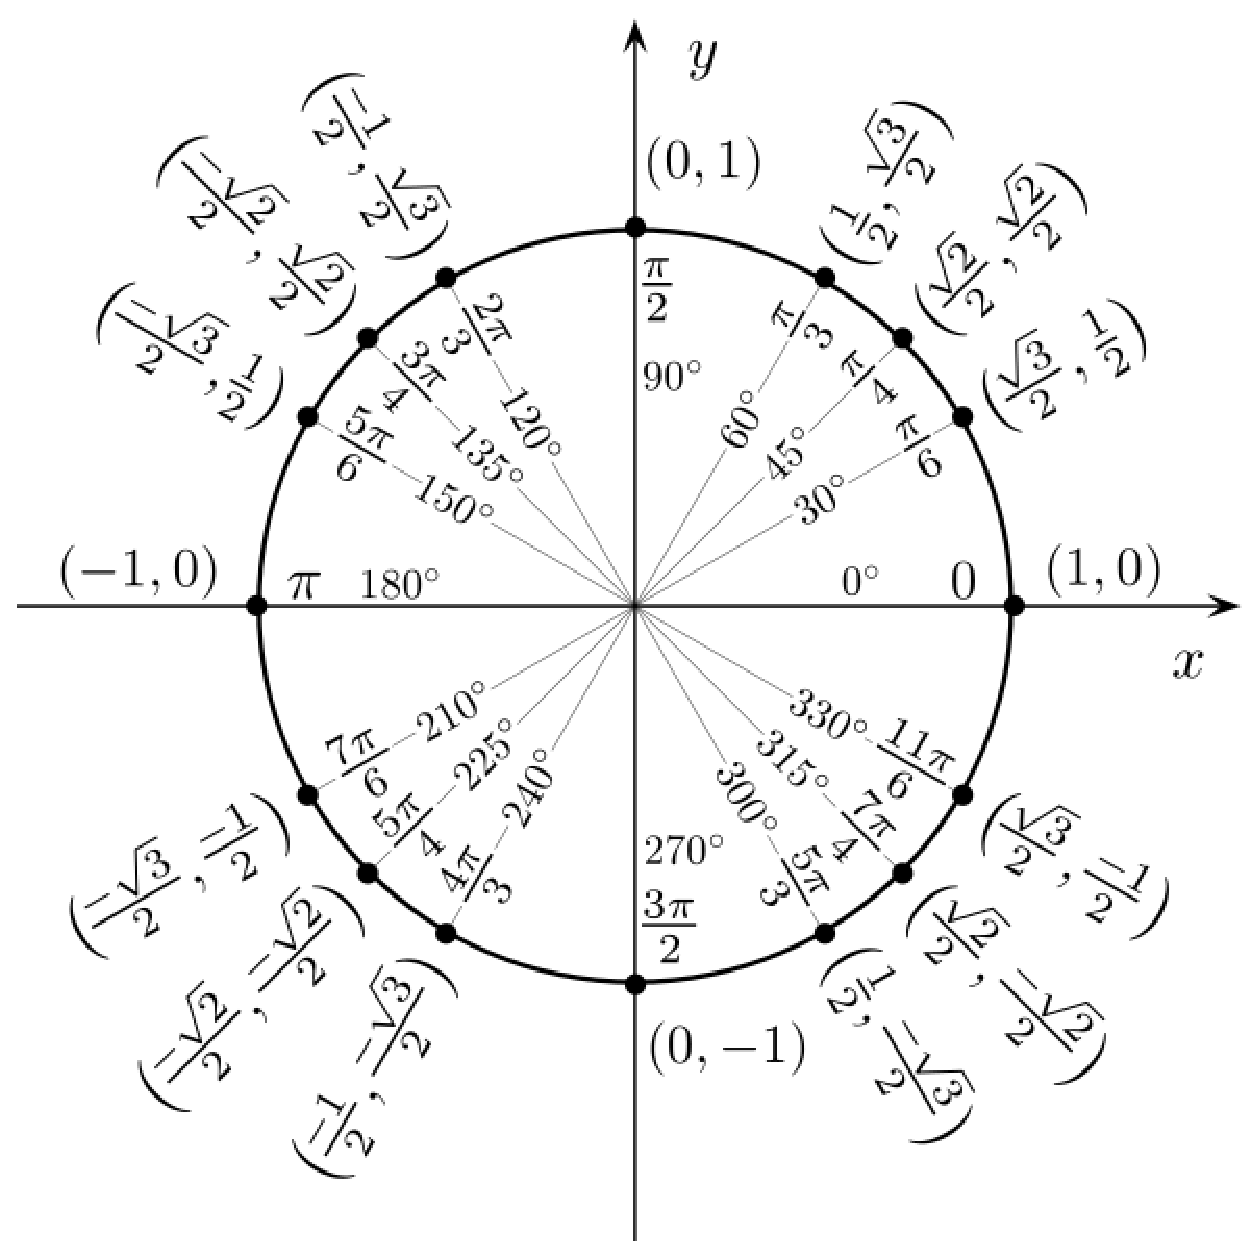
\includegraphics[width=4.0in]{UnitCircle2}
\end{center}
\bigskip

\vfill
\eject

\begin{large}
\textbf{Bessel Functions}
\end{large}
\medskip

\begin{center}
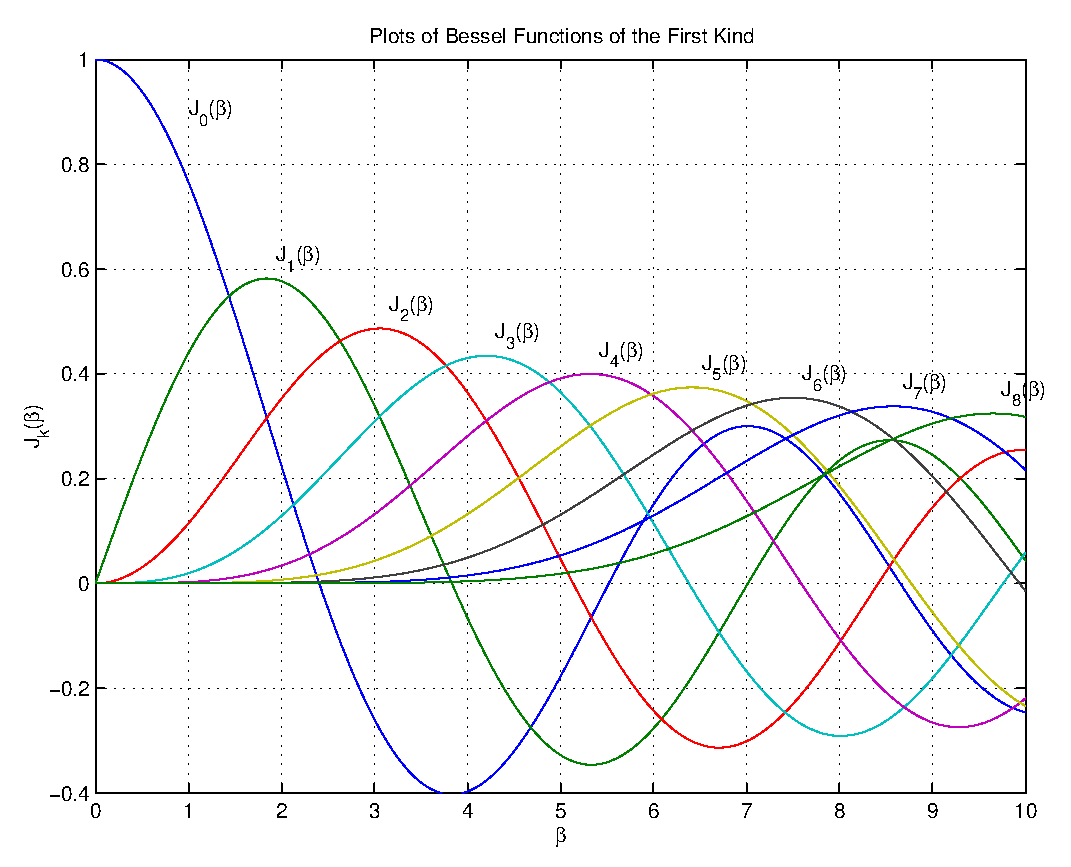
\includegraphics[width=6.0in]{jkbeta1}
\end{center}
\medskip

\noindent $\displaystyle J_k(\beta)=\frac{1}{2\pi}\int_{-\pi}^{\pi}
e^{j(\beta\sin x-k x)}\,dx\>,$ Bessel function of 1'st kind, order $k$.
\bigskip

\noindent Properties:
\medskip

\begin{tabular}{rl}
1.&$J_k(\beta)=J^*_k(\beta)$\\[6pt]
2.&$J_{-k}(\beta)=(-1)^k\, J_k(\beta)$\\[6pt]
3.&$\displaystyle\sum_{k=-\infty}^{\infty} J_k^2(\beta)=1$
\end{tabular}

\vfill
\eject

\begin{large}
\textbf{ASCII Code}
\end{large}
\medskip
\bigskip

\noindent
\begin{tabular}
  {|c!{\vrule width 1pt}c|c|c|c|c|c|c|c|}
  \hline
  \multicolumn{9}{|c|}{\phantom{m}}\\[-9pt]
  \multicolumn{9}{|c|}{\textbf{\phantom{i}7-Bit ASCII (American Standard Code for Information Interchange)\phantom{i}}}\\[4pt]
  \hline
  \phantom{m}&&&&&&&&\\[-10pt]
  &\texttt{000...}&\texttt{001...}&\texttt{010...}&\texttt{011...}
  &\texttt{100...}&\texttt{101...}&\texttt{110...}&\texttt{111...}\\[2pt]
  \noalign{\hrule height1pt}
  \phantom{m}&&&&&&&&\\[-10pt]
  \texttt{..0000}&\textsl{NUL}&\textsl{DLE}&\texttt{\textsl{SP}}&\texttt{\symbol{"30}}
  &\texttt{\symbol{"40}}&\texttt{\symbol{"50}}&\texttt{\symbol{"60}}&\texttt{\symbol{"70}}\\[2pt]
  \hline
  \phantom{m}&&&&&&&&\\[-10pt]
  \texttt{..0001}&\textsl{SOH}&\textsl{DC1}&\texttt{\symbol{"21}}&\texttt{\symbol{"31}}
  &\texttt{\symbol{"41}}&\texttt{\symbol{"51}}&\texttt{\symbol{"61}}&\texttt{\symbol{"71}}\\[2pt]
  \hline
  \phantom{m}&&&&&&&&\\[-10pt]
  \texttt{..0010}&\textsl{STX}&\textsl{DC2}&\texttt{\symbol{"22}}&\texttt{\symbol{"32}}
  &\texttt{\symbol{"42}}&\texttt{\symbol{"52}}&\texttt{\symbol{"62}}&\texttt{\symbol{"72}}\\[2pt]
  \hline
  \phantom{m}&&&&&&&&\\[-10pt]
  \texttt{..0011}&\textsl{ETX}&\textsl{DC3}&\texttt{\symbol{"23}}&\texttt{\symbol{"33}}
  &\texttt{\symbol{"43}}&\texttt{\symbol{"53}}&\texttt{\symbol{"63}}&\texttt{\symbol{"73}}\\[2pt]
  \hline
  \phantom{m}&&&&&&&&\\[-10pt]
  \texttt{..0100}&\textsl{EOT}&\textsl{DC4}&\texttt{\symbol{"24}}&\texttt{\symbol{"34}}
  &\texttt{\symbol{"44}}&\texttt{\symbol{"54}}&\texttt{\symbol{"64}}&\texttt{\symbol{"74}}\\[2pt]
  \hline
  \phantom{m}&&&&&&&&\\[-10pt]
  \texttt{..0101}&\textsl{ENQ}&\textsl{NAK}&\texttt{\symbol{"25}}&\texttt{\symbol{"35}}
  &\texttt{\symbol{"45}}&\texttt{\symbol{"55}}&\texttt{\symbol{"65}}&\texttt{\symbol{"75}}\\[2pt]
  \hline
  \phantom{m}&&&&&&&&\\[-10pt]
  \texttt{..0110}&\textsl{ACK}&\textsl{SYN}&\texttt{\symbol{"26}}&\texttt{\symbol{"36}}
  &\texttt{\symbol{"46}}&\texttt{\symbol{"56}}&\texttt{\symbol{"66}}&\texttt{\symbol{"76}}\\[2pt]
  \hline
  \phantom{m}&&&&&&&&\\[-10pt]
  \texttt{..0111}&\textsl{BEL}&\textsl{ETB}&\texttt{\symbol{"27}}&\texttt{\symbol{"37}}
  &\texttt{\symbol{"47}}&\texttt{\symbol{"57}}&\texttt{\symbol{"67}}&\texttt{\symbol{"77}}\\[2pt]
  \hline
  \phantom{m}&&&&&&&&\\[-10pt]
  \texttt{..1000}&\textsl{BS}&\textsl{CAN}&\texttt{\symbol{"28}}&\texttt{\symbol{"38}}
  &\texttt{\symbol{"48}}&\texttt{\symbol{"58}}&\texttt{\symbol{"68}}&\texttt{\symbol{"78}}\\[2pt]
  \hline
  \phantom{m}&&&&&&&&\\[-10pt]
  \texttt{..1001}&\textsl{HT}&\textsl{EM}&\texttt{\symbol{"29}}&\texttt{\symbol{"39}}
  &\texttt{\symbol{"49}}&\texttt{\symbol{"59}}&\texttt{\symbol{"69}}&\texttt{\symbol{"79}}\\[2pt]
  \hline
  \phantom{m}&&&&&&&&\\[-10pt]
  \texttt{..1010}&\textsl{LF}&\textsl{SUB}&\texttt{\symbol{"2A}}&\texttt{\symbol{"3A}}
  &\texttt{\symbol{"4A}}&\texttt{\symbol{"5A}}&\texttt{\symbol{"6A}}&\texttt{\symbol{"7A}}\\[2pt]
  \hline
  \phantom{m}&&&&&&&&\\[-10pt]
  \texttt{..1011}&\textsl{VT}&\textsl{ESC}&\texttt{\symbol{"2B}}&\texttt{\symbol{"3B}}
  &\texttt{\symbol{"4B}}&\texttt{\symbol{"5B}}&\texttt{\symbol{"6B}}&\texttt{\symbol{"7B}}\\[2pt]
  \hline
  \phantom{m}&&&&&&&&\\[-10pt]
  \texttt{..1100}&\textsl{FF}&\textsl{FS}&\texttt{\symbol{"2C}}&\texttt{\symbol{"3C}}
  &\texttt{\symbol{"4C}}&\texttt{\symbol{"5C}}&\texttt{\symbol{"6C}}&\texttt{\symbol{"7C}}\\[2pt]
  \hline
  \phantom{m}&&&&&&&&\\[-10pt]
  \texttt{..1101}&\textsl{CR}&\textsl{GS}&\texttt{\symbol{"2D}}&\texttt{\symbol{"3D}}
  &\texttt{\symbol{"4D}}&\texttt{\symbol{"5D}}&\texttt{\symbol{"6D}}&\texttt{\symbol{"7D}}\\[2pt]
  \hline
  \phantom{m}&&&&&&&&\\[-10pt]
  \texttt{..1110}&\textsl{SO}&\textsl{RS}&\texttt{\symbol{"2E}}&\texttt{\symbol{"3E}}
  &\texttt{\symbol{"4E}}&\texttt{\symbol{"5E}}&\texttt{\symbol{"6E}}&\texttt{\symbol{"7E}}\\[2pt]
  \hline
  \phantom{m}&&&&&&&&\\[-10pt]
  \texttt{..1111}&\textsl{SI}&\textsl{US}&\texttt{\symbol{"2F}}&\texttt{\symbol{"3F}}
  &\texttt{\symbol{"4F}}&\texttt{\symbol{"5F}}&\texttt{\symbol{"6F}}&\textsl{DEL}\\[2pt]
  \hline
\end{tabular}

\end{document}


\subsection{Phasors}

\noindent
\bigskip

\begin{center}
\includegraphics[width=6.5in]{circuit01}
\end{center}

\[\renewcommand{\arraystretch}{1.15}
\begin{array}{ll}
\mbox{line 1} & \\
\mbox{line 2} &
\end{array}\]

\[p(t)=\displaystyle\left\{\begin{array}{ll}1\>,&-T_B/2\le t<T_B/2\>,\\
0\>,&\mbox{otherwise}\>.\end{array}\right.\]

\symbol{"5F}

\noindent\begin{boxedverbatim}
u = [0 1 2 3 4 5];
\end{boxedverbatim}

\begin{center}
\begin{tabular}{lll}
Particle&\quad Mass&\quad Charge\\[3pt]
\noalign{\hrule height0.7pt}
\phantom{m}&&\\[-10pt]
Electron&\quad$m_E=9.10939\times 10^{-31}$ kg&\quad$q_E=-1.60218\times 10^{-19}$ C\\[0pt]
\end{tabular}
\end{center}

\begin{center}
\begin{tabular}{!{\vrule width 1pt}c|c|c!{\vrule width 1pt}}
\noalign{\hrule height1pt}
\multicolumn{3}{!{\vrule width 1pt}c!{\vrule width 1pt}}{\phantom{m}}\\[-10pt]
\multicolumn{3}{!{\vrule width 1pt}c!{\vrule width 1pt}}
{\strut\textbf{Flat-Top PAM Signal}, Baud Rate $F_B$}\\[3pt]
\hline
\phantom{m}&&\\[-11pt]
\phantom{m}$f_1$\phantom{m}&$\phantom{m}f_2\phantom{m}$&$P_x(f_1,f_2)/P_x$ in \%\\[3pt]
\noalign{\hrule height1pt}
\phantom{m}&&\\[-10pt]
$-F_B$&$F_B$&90.30\%\\[2pt]
\noalign{\hrule height1pt}
\end{tabular}
\end{center}

\noindent\begin{boxedverbatim}
disp(['pi is equal to ' num2str(pi,10) ' with 10-digit accuracy'])
\end{boxedverbatim}
\bigskip
